\chapter{PROTOCOLOS DE COMUNICAÇÃO}

A comunicação envolve a troca de uma série de mensagens entre duas entidades. Cada
uma das partes envolvidas no diálogo supõe uma série de premissas a respeito das
informações transmitidas e recebidas, como por exemplo a linguagem e o meio de
transmissão. Caso os envolvidos não concordem em relação a estas premissas, não
será possível estabelecer uma comunicação adequada.

Restrições a respeito do formato, meios de transmissão, e ações a serem tomadas no
envio e recebimento de mensagens são definidas por meio de protocolos. A partir do
momento em que duas entidades seguem o mesmo protocolo, pode-se garantir que a
comunicação será estabelecida. Assim como qualquer outra entidade, componentes de
\textit{hardware} e \textit{software} também estão sujeitos a protocolos de
comunicação \cite{kurose2012}.

Também é importante indicar que protocolos definem apenas as regras envolvidas em
uma troca de mensagens. Desde que as entidades cumpram as restrições, portanto
adotando a interface proposta, a estratégia de implementação se torna arbitrária.



\section{SUÍTES DE PROTOCOLOS}

No contexto da computação, redes de comunicação são construídas com diferentes
tecnologias de acordo com necessidades e restrições específicas, o que prejudica a
capacidade de intercomunicação entre dispositivos \cite{comer2000}. A Internet, por
exemplo, é uma coleção de redes menores que eventualmente utilizam tecnologias
diferentes, como é o caso de linhas telefônicas, e transmissão a rádio
\cite{tanenbaum2010}. Um desafio diferente é alcançar a intercomunicação em um
sistema complexo como tal, onde as redes que o compõem utilizam seus próprios
protocolos, desta vez específicos ao meio de transmissão.

De acordo com \cite{comer2000}, existem duas observações fundamentais ao projeto de
redes de comunicação:

\begin{enumerate}
  \item{Não existe nenhuma tecnologia de rede capaz de satisfazer a todas as
        restrições. Portanto, é natural que existam diferentes tecnologias para
        diferentes contextos e necessidades;}
  \item{Usuários desejam intercomunicação universal.}
\end{enumerate}

A intercomunicação pode ser implementada tanto no nível das aplicações quanto no
nível da rede. A implementação no nível da aplicação deve prever as especificidades
das tecnologias de rede envolvidas, o que a torna complexa ou até mesmo impossível
para alguns sistemas, como a Internet. A implementação no nível de rede é mapeada
a partir do \textit{hardware} e prioriza o transporte de pacotes menores entre
entidades sem a necessidade de programas intermediários. Neste caso, não há
necessidade em compreender as aplicações em comunicação, que por sua vez podem ser
implementadas com maior flexibilidade a partir de um nível de abstração mais elevado
\cite{comer2000}.

A intercomunicação no nível de rede (ou simplesmente internet \cite{comer2000}) é
baseada na adoção de um modelo de camadas no projeto das rede de computadores. Com
esta metodologia os protocolos são organizados em uma hierarquia vertical, de acordo
com seus objetivos. Cada camada utiliza os serviços do nível anterior e oferece
novas funcionalidades a partir de um nível de abstração mais elevado. A interface
entre as camadas deve ser bem definida, o que significa que componentes que
implementam um padrão não precisam se atentar às restrições dos protocolos das
camadas subjacentes \cite{kurose2012}.

O TCP/IP, também conhecido como a suíte de protocolos da Internet, surgiu para
satisfazer as necessidades de interoperabilidade em um sistema de redes heterogêneo,
as quais não eram satisfeitas por nenhum dos padrões que existiam até então. O
conjunto de protocolos da Internet trabalha cooperativamente em um modelo de
camadas, tornando possível a comunicação entre redes distintas e interconectadas
\cite{comer2000}.

Em uma hierarquia de camadas, as mensagens são enviadas sucessivamente da camada
mais superior até a camada mais inferior durante a transmissão, o inverso do que
acontece no recebimento. As camadas mais inferiores do transmissor e destinatário
são conectadas entre si através de um meio de transmissão arbitrário, o que leva
garante abstração do meio físico às camadas superiores.

\begin{figure}[h]
	\centering
		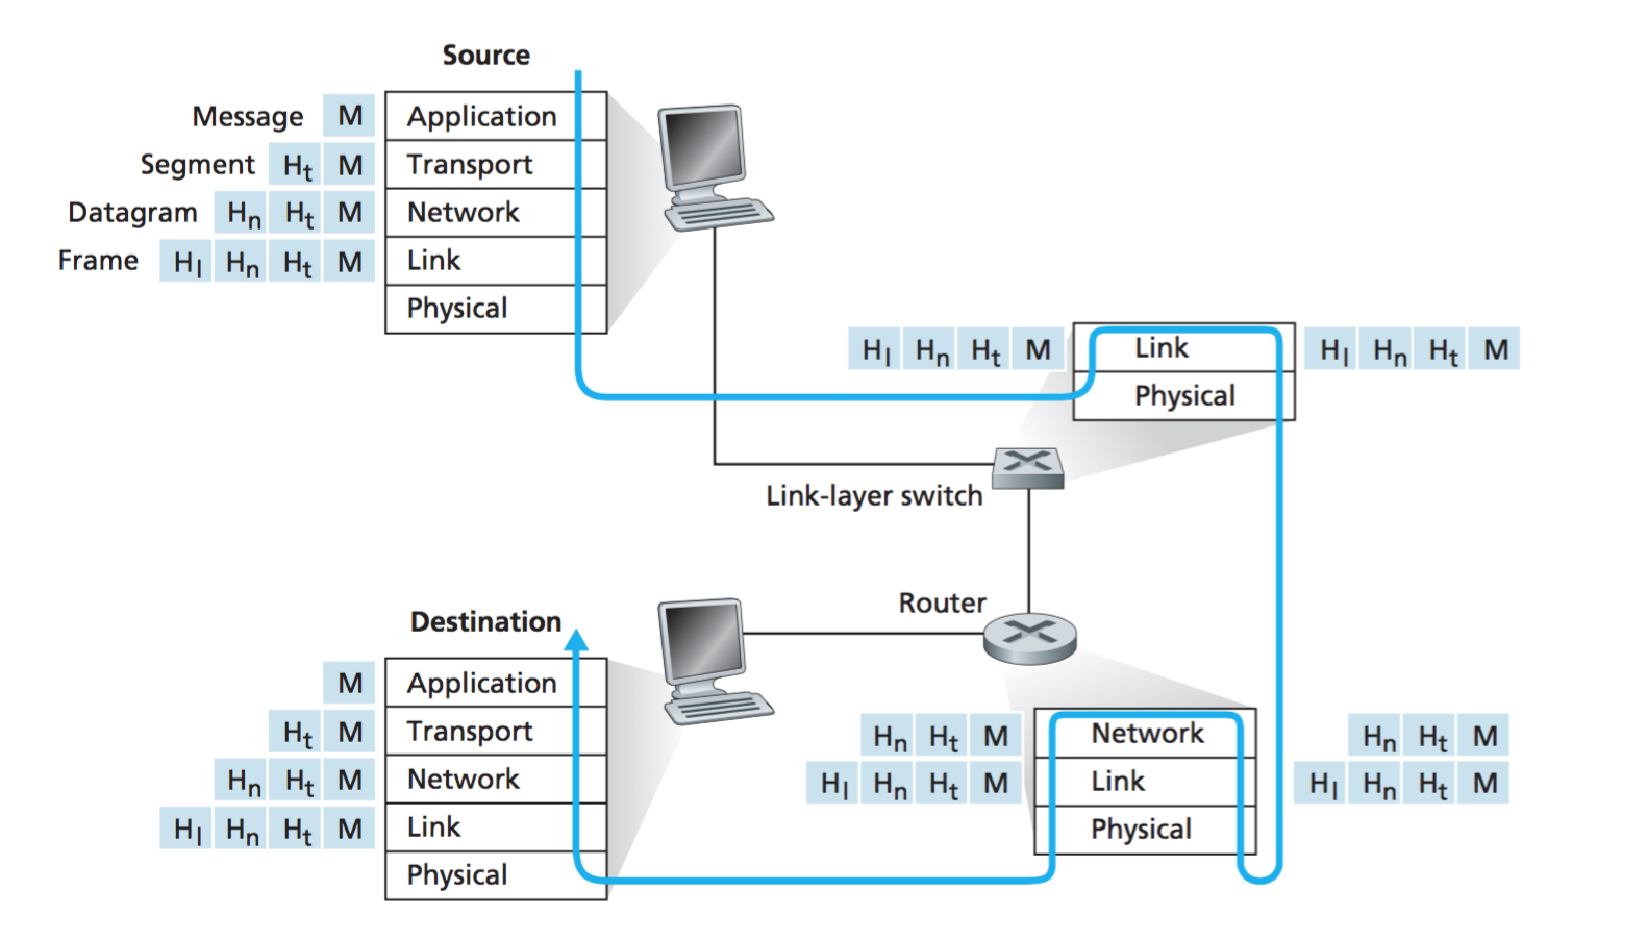
\includegraphics[keepaspectratio=true,scale=0.6]{figuras/encapsulamento.eps}
	\caption{Encapsulamento de mensagens em um modelo de camadas \cite{kurose2012}}
	\label{fig:encapsulamento}
\end{figure}

Cada camada trabalha sobre pacotes, adicionando informações necessárias (cabeçalhos)
para o seu trabalho no envio, e removendo-os no recebimento. Os pacotes consistem em
um conjunto de dados transportados (\textit{payload}) e um cabeçalho, utilizado
apenas no nível da mesma camada. Os cabeçalhos permitem que as camadas trabalhem
em cooperação, mantendo um diálogo consistente com o protocolo do nível respectivo
das entidades envolvidas na comunicação. A figura \ref{fig:encapsulamento} mostra
este processo no contexto do TCP/IP.

% Encontrar um exemplo ou usar o OStatus + referência
Apesar deste processo descrever a interação entre os protocolos organizados em um
modelo de camadas, uma estratégia semelhante é utilizada em outras suítes. Uma
família de protocolos da camada de aplicação, por exemplo, não segue nenhum dos
modelos de camadas de redes de comunicação, mas ainda assim utiliza os conceitos de
hierarquia e encapsulamento para garantir interoperabilidade e cumprir uma tarefa
específica em conjunto.



\section{PADRONIZAÇÃO DE PROTOCOLOS}

A definição de protocolos é apenas o primeiro passo para a intercomunicação de
sistemas. Se não existir um acordo a respeito da especificação utilizada será mais
difícil estabelecer a comunicação entre serviços \cite{kurose2012}. A padronização
garante o estabelecimento deste acordo.

A partir do momento em que uma série de entidades entra em consenso a respeito da
especificação de um protocolo, estabelece-se um padrão \textit{de facto}. A
iniciativa de padronização também pode surgir através de entidades regulamentadoras,
como a Organização Internacional para a Padronização (ISO), ou a \textit{Internet
Engineering Task Force} (IETF), o que leva ao estabelecimento padrões \textit{de
jure} \cite{tanenbaum2010}.

O conceito de efeito de rede indica que a adoção de um protocolo se torna mais
valiosa à medida que um maior número de entidades também o utilize
\cite{liebowitz1998}. Justifica-se portanto o interesse em incentivar a padronização
de protocolos.

O processo de definição de novos padrões \textit{de jure} depende da entidade
regulamentadora relacionada, e ocasionalmente parte de padrões \textit{de facto} já
utilizados na comunidade. Geralmente uma especificação é proposta, discutida, e
revisada pela entidade antes de se tornar um padrão, o que no caso da ISO pode levar
de seis meses a alguns anos \cite{tanenbaum2010}.

Propostas e padrões estabelecidos devem ser documentados de alguma forma. A IETF
adota o formato de \textit{Request for Comments} (RFC), publicações que descrevem
completamente uma especificação, e estão disponíveis a consulta pela comunidade.

Uma proposta deve cumprir uma série de requisitos antes de ser endossado por uma
organização. No caso da IETF, propostas passam por diferentes níveis de maturidade
até alcançar a categoria de padrão. Cada um destes níveis pode ser alcançado ao
satisfazer as recomendações de um grupo da comunidade, o que acontece durante o
processo de padronização. Um exemplo de requisito deste processo é a existência de
uma prova técnica de conceito, como demonstração de interoperabilidade entre duas ou
mais implementações distintas \cite{rfc1280}.


\subsection{Simple Mail Transfer Protocol}

A troca de mensagens na internet é um problema recorrente, envolve as questões de
interoperabilidade entre redes, e depende da adoção de padrões para a comunicação
entre serviços. O esforço de especificação acontece desde a década de 70 com o
\textit{Mail Box Protocol}, e continua desde a definição do \textit{Simple Mail
Transfer Protocol}.

O SMTP é um protocolo para o transporte e entrega de mensagens de e-mail entre
processos. A especificação garante que a troca de mensagens aconteça entre clientes
que se localizam em redes diferentes, o que permite a construção de um serviço que
funcione de maneira confiável sobre a internet \cite{rfc2821}. Trata-se de um
protocolo amplamente adotado e formalmente padronizado desde 1982, portanto
interessante para ser analisado no contexto do estabelecimento de padrões.

Caracterizado como um protocolo orientado a conexões entre clientes e servidores, ou
transmissores e receptores, o SMTP é guiado por uma série de comandos predefinidos.
Os servidores também são responsáveis por retransmitir mensagens, caso não sejam os
destinatários finais \cite{kurose2012}.

A troca de mensagens geralmente acontece em um único salto após o estabelecimento de
uma conexão orientada entre o remetente e o destinatário. A retransmissão de
mensagens é uma alternativa que deve ser explicitamente utilizada, por exemplo em
casos em que um usuário moveu sua caixa de e-mails de um servidor para outro e
deseja receber as mensagens no seu novo endereço.

\begin{figure}[h]
	\centering
		\includegraphics[keepaspectratio=true,scale=0.6]{figuras/smpt_internet.eps}
	\caption{Uma visão geral de um sistema de e-mails \cite{kurose2012}}
	\label{fig:smtpInternet}
\end{figure}

Como pode ser visto na figura \ref{fig:smtpInternet}, o SMTP é um protocolo
intermediário entre servidores de e-mail que alternam entre os papéis de transmissor
e receptor. Cada um destes servidores fornece a seus próprios clientes, constituindo
sistemas menores onde a interação não é necessariamente coberta pela especificação
do SMTP.

Cada um destes sistemas intermediários não é necessariamente compatível, visto que a
comunicação entre o servidor e o usuário depende das aplicações envolvidas, e
eventualmente utiliza outros padrões, como por exemplo POP3 ou IMAP no gerenciamento
de caixas de e-mail pessoais \cite{tanenbaum2010}. A organização deste esquema é um
exemplo de como a utilização de um padrão possibilita a comunicação em um sistema
heterogêneo.

Ainda levando em consideração a organização descentralizada apresentada pela figura
\ref{fig:smtpInternet}, pode-se indicar a semelhança com o formato de sistemas
federados. Qualquer novo sistema capaz de implementar a especificação do SMTP
torna-se parte da federação, onde a heterogeneidade entre os sistemas é
completamente transparente para os usuários do serviço.

O SMTP foi definido em publicações da IETF, tendo sido proposto com base em
especificações anteriores. Trata-se de um padrão \textit{de jure} aberto, endossado
por uma organização e então adotado pelo mercado.



\section{PROTOCOLOS DE FEDERAÇÃO}

% TODO
% seção de fatores que dificultam a padronização da federação?

A inexistência de um protocolo padrão para a federação de mídias sociais dificulta
o desenvolvimento de aplicações interoperáveis. São enfrentados os mesmos problemas
identificados na intercomunicação de redes heterogêneas, já que os desenvolvedores
solucionam os problemas com tecnologias diferentes, de acordo com as próprias
restrições e necessidades.

Ainda que exista uma tendência da comunidade em adotar propostas de protocolos, o
que pôde ser observado no caso do projetos OStatus e Diaspora, abordagens
alternativas naturalmente serão desenvolvidas. Já que cada projeto conta com suas
próprias restrições, a ausência de um padrão leva à segmentação da adoção por parte
dos desenvolvedores, o que prejudica o efeito de rede e impede o surgimento de um
padrão \textit{de facto}.

Ao discutir a padronização da federação é interessante não só analisar o esforço da
comunidade em discutir e adotar propostas ainda não completamente estabelecidas,
como também identificar as questões que impediram um acordo.


\subsection{OSTATUS}

O OStatus é um conjunto de protocolos que permite a interação em tempo real entre
redes redes sociais distintas. Foi inicialmente proposto por Evan Prodromou para a
implementação no StatusNet, que posteriormente deu origem ao projeto Gnu
\textit{social}.

Até certo ponto, tecnologias como o Atom e RSS permitem a interação entre sistemas,
mais especificamente no compartilhamento de conteúdo. No entanto, são restritas no
que diz respeito a interação em tempo real, problema que o OStatus propõe resolver
combinando \textit{feeds} Atom com uma série de outros mecanismos.

A especificação do OStatus propõe a utilização das tecnologias listadas a seguir.

\begin{itemize}
  \item{PubSubHubbub: mecanismo de inscrição e submissão}
  \item{WebFinger: descoberta de identidade}
  \item{Activity Streams: representação de atividades de usuários em redes sociais}
  \item{Salmon: descentralização de trocas de mensagens}
\end{itemize}

O projeto obteve visibilidade na comunidade, contando com uma das maiores
iniciativas de padronização. O OStatus chegou a se tornar alvo de um grupo de
trabalho da W3C em 2012, uma das maiores organizações de padronização para a
\textit{web}. Apesar disto, o grupo não apresentou avanços desde então, e o
desenvolvimento do projeto está estagnado.

\subsubsection{PubSubHubbub}

O PubHubSub especifica sistemas distribuídos para publicação e assinatura de
conteúdos. A ideia é que serviços possam se inscrever em diretórios centrais (ou
\textit{hubs}), expressando o interesse em receber as atualizações em tempo real.

Serviços inscritos devem identificar o tópico desejado através de URLs, e oferecer
um servidor disponível pela internet para que a notificação possa ser realizada.
É de responsabilidade dos produtores de conteúdo notificar o \textit{hub} em cada
nova publicação, que por sua vez são responsáveis por divulgar para cada um dos
indivíduos inscritos.

A comunicação dos \textit{hubs} com as entidades que publicam e consomem os
conteúdos acontecem sobre HTTP, cada uma destas identificadas por endereços URL. As
notificações são baseadas na execução de trechos arbitrários de código ativados a
partir de \textit{endpoints} URL, seguindo a ideia de \textit{webhooks}.

\subsubsection{WebFinger}

O WebFinger é um protocolo de descoberta de identidade que soluciona o problema do
compartilhamento de informações de usuários entre servidores remotos \cite{rfc7033}.
A proposta é que a partir de um atributo identificador de um usuário e o endereço do
seu servidor de origem, seja possível garantir sua existência e recuperar suas
informações públicas.

A especificação do WebFinger propõe que todos os recursos possam ser identificados
por uma URL, e que todas as solicitações e respostas sejam realizadas através de
requisições HTTP. Servidores que forneçam informações através do WebFinger devem
responder aos \textit{endpoints} definidos no protocolo com objetos JSON. Servidores
que pretendam consumir tais informações precisam conhecer apenas a URL do recurso de
interesse, o que pode ser encontrado a partir do identificador do usuário e do
domínio do servidor de origem (em um processo que pode ser classificado como LRDD
\cite{lrdd2010}). 

\subsubsection{Activity Streams}

O Activity Streams é uma especificação que propõe um formato para a representação
das atividades dos usuários em uma rede social. O objetivo é facilitar o consumo
destas ações para o resto da rede, e por consequência a integração de aplicações.

A especificação mais atual do Activity Streams propõe a representação em formato
JSON, incluindo uma série de propriedades que identificam a ação, o usuário
responsável, e a entidade alvo. Especificações mais antigas utilizam o padrão Atom,
com restrições semelhantes em relação ao conteúdo e formato das mensagens. O OStatus
adota o protocolo especificado em Atom para o envio de entradas de Activity Streams.

O padrão trata apenas da representação das mensagens, dependendo de outros
mecanismos para a distribuição das atividades. Geralmente são utilizadas APIs ou
\textit{feeds} em conjunto com mecanismos de inscrição.

\subsubsection{Salmon}

Combinar soluções como Atom e PubHubSub permite que conteúdos sejam publicados e
atualizados em tempo real. No entanto, a partir do ponto em que um conteúdo pode ser
consumido a partir de um número arbitrário de serviços, deve-se investir esforço
para garantir que o seu estado (que inclui todas as atividades relacionadas) seja o
mesmo em toda a rede.

O objetivo do Salmon é descentralizar a capacidade de contribuir com o estado de um
conteúdo, ainda que mantendo a sua consistência em todas as entidades consumidoras.
Mais precisamente, especificação a troca de mensagens entre entidades consumidoras
e o servidor de origem de uma publicação, definindo um formato para as mensagens, e
um fluxo para a agregação das atividades.

Um servidor que implemente o protocolo deve incluir a URL de um \textit{endpoint}
capaz de processar mensagens Salmon, enviadas para este endereço por qualquer
serviço interessado em contribuir com o estado de uma publicação. Uma mensagem
Salmon se trata de uma nova entrada no \textit{feed}, codificada em \textit{base64},
envolta por outra estrutura XML assinada digitalmente. Cabe ao servidor de origem
publicar ou não estas novas entradas, de acordo com suas próprias políticas.

\subsubsection{Fluxo do OStatus}

Cada protocolo utilizado na especificação do OStatus possui uma responsabilidade
específica no fluxo de comunicação. A [[[referenciar o diagrama]]] apresenta um
cenário em que dois usuários de servidores distintos interagem através deste fluxo,
apontando o papel de cada um dos mecanismos intermediários.

% diagrama do workflow do OStatus

\begin{enumerate}
  \item{O usuário A descobre o endereço do servidor de origem do usuário B através
        do WebFinger}
  \item{O usuário A se inscreve no \textit{feed} público através do PubHubSub
        através do endereço obtido}
  \item{O usuário A envia uma nova entrada no formato Activity Streams através de
        uma mensagem Salmon para o usuário B, notificando-o da ação}
  \item{O servidor do usuário B atualiza sua lista de seguidores. Eventualmente, o
        usuário B publica um novo conteúdo, notificando os inscritos através do
        PubHubSub}
  \item{O usuário A recebe o \textit{feed} atualizado através do PubHubSub, e decide
        publicar um novo comentário. Uma nova entrada no \textit{feed} é criada em
        formato Activity Streams, e novamente enviada ao servidor original através
        de uma mensagem Salmon}
  \item{O servidor do usuário B recebe a mensagem, e registra um novo comentário,
        atualizando seu \textit{feed} e notificando novamente os seus inscritos}
\end{enumerate}

\subsubsection{Estado do padrão}

O projeto OStatus deu um passo importante em direção à padronização com a criação do
grupo de trabalho na W3C. No entanto, a comunidade não conseguiu entrar em consenso
em relação às decisões do protocolo, principalmente no que diz respeito à
privacidade.

Não exitem avanços no projeto nos últimos anos, e o grupo de trabalho da W3C não
produziu nenhum relatório desde que foi criado. Em 2012 o fundador do projeto, Evan
Prodromou, anunciou o desenvolvimento do \textit{pump.io}, outro protocolo de
federação, abandonando o desenvolvimento do OStatus.

Ao mesmo tempo em que não existia comunidade ativa para a evolução do projeto, parte
das tecnologias relacionadas continuou a ser mantida, o que contribui para o seu
estado de obsolescência. O Activity Streams, por exemplo, já conta com uma segunda
especificação que suporte tecnologia JSON, enquanto o OStatus ainda considera a
especificação baseada em Atom.


\subsection{Diaspora}

O projeto Diaspora surgiu com a intenção de implementar o conceito de redes sociais
descentralizadas em resposta aos problemas de liberdade e privacidade encontrados em
plataformas sociais privadas. Sua primeira versão foi lançada em Setembro de 2010
como fruto de uma campanha de financiamento coletivo, passando a ser completamente
governado pela comunidade a partir de Agosto de 2012.

A proposta dos desenvolvedores é evitar a centralização de conteúdo, portanto a
falta de controle sobre as informações, construindo uma rede de instâncias pessoais
da plataforma, ou \textit{pods}. Cada servidor Diaspora reúne apenas as informações
dos seus próprios usuários, mas em cooperação com outros \textit{pods} possibilita a
interação em uma rede federada.

O protocolo de federação do Diaspora foi definido para convergir com o OStatus assim
que o último passe a suportar o conceito de privacidade limitada, o que nunca
aconteceu. A implementação leva em consideração a troca de mensagens em formato XML,
respeitando alguns conceitos básicos como a existência de usuários remotos e
atualização remota e retransmissão.

\subsubsection{Usuários Remotos}

Um conceito fundamental para a implementação de redes federadas é considerar a
existência de usuários remotos. A maioria das aplicações só possui o conceito de
usuários locais, que estão diretamente autenticados no serviço e possuem todas as
informações na base de dados local. No entanto, ao possibilitar a interação com
usuários de outras redes, usuários externos ao sistema precisam ser explicitamente
considerados na implementação das funcionalidades.

O Diaspora conceitualiza seus usuários em locais e externos. Enquanto usuários locais
respeitam a definição tradicional, os usuários externos interagem com a aplicação
através dos mecanismos de federação. É importante prever a existência de usuários
externos na modelagem de sistemas. Por este motivo, implementar federação em
aplicações já consolidadas pode exigir um certo esforço de refatoração. % ref?

\subsubsection{Capacidade de Retransmissão}

A retransmissão é essencial em sistemas federados, visto que interações em uma rede
eventualmente devem afetar \textit{pods} relacionados. A restrição implementada pelo
Diaspora indica que todas as notificações neste contexto sejam entregues tanto aos
usuários locais quanto aos usuários remotos. Adicionalmente, a notificação de
usuários locais não deve depender da resposta dos demais \textit{pods}.

Em configurações de integração mais complexas, a capacidade de retransmissão passa a
ser um requisito essencial para a troca de mensagens. Considere uma situação
hipotética em que \textit{pods} \textbf{A} e \textbf{B} são federados com o
\textit{pod} \textbf{C}, mas não entre si. Qualquer modificação em um conteúdo de
\textbf{C} compartilhado com \textbf{A} e \textbf{B} deve afetar os três
\textit{pods}. No entanto, se a modificação partir de \textbf{A}, há uma dificuldade
em notificar \textbf{B}, visto que o \textit{pod} em questão só reconhece a
existência de \textbf{C}. A solução defendida pela implementação do Diaspora é que
\textbf{C} retransmita a notificação para todos os \textit{pods} com os quais o
conteúdo seja compartilhado. Isso garante que todos os sistemas federados envolvidos
em uma interação sejam notificados, contribuindo com consistência das informações.

\subsubsection{Troca de Mensagens}

O Diaspora define um conjunto de mensagens que delimitam as possíveis interações
entre \textit{pods}.

\begin{itemize}
  \item{Compartilhamento de informações}
  \item{Publicações de conteúdo}
  \item{Comentários e reações a publicações}
  \item{Mensagens privadas}
\end{itemize}

A troca de mensagens segue a definição do protocolo Diaspora, que utiliza um
subconjunto do protocolo Salmon. De modo geral, restringe como a mensagem deve ser
construída e enviada para o \textit{endpoint} Salmon do \textit{pod} de destino. 

\subsubsection{Fluxo do Protocolo Diaspora}

O protocolo Diaspora cobre tanto a descoberta de identidades entre os servidores,
quanto o envio e recebimento de informações. De forma análoga ao OStatus, parte da
implementação também utiliza outros protocolos, como o WebFinger, o Activity Streams
e o Salmon. Uma outra especificação implementada é o hCard, que trata da
representação das informações de um usuário em formato HTML ou XML. % ref hCard

O diagrama da [[[figura]]] representa o fluxo de uma interação entre dois usuários de
\textit{hubs} distintos.

% diagrama do workflow do Diaspora

% revisar o fluxo do protocolo

\begin{enumerate}
  \item{O usuário A deseja seguir o \textit{feed} do usuário B localizado em outro
        \textit{hub} do Diaspora. O primeiro passo é descobrir o WebFinger de B
        através das informações de seu \textit{hub}, e solicitar o seu perfil}
  \item{O \textit{hub} do usuário B responde com o perfil WebFinger de B, que além
        de suas informações inclui uma URL do seu \textit{feed} em Activity Streams,
        e uma chave pública RSA para a troca de mensagens}
  \item{O usuário A cria uma nova mensagem solicitando o compartilhamento e a envia
        por meio de Salmon para o usuário B}
  \item{O usuário B começa a compartilhar suas publicações com A, enviando uma nova
        mensagem Salmon a cada nova publicação}
  \item{O usuário A recebe a nova publicação, e decide enviar um novo comentário.
        Uma nova mensagem Activity Streams é construída e enviada por meio de Salmon
        para o \textit{hub} original}
  \item{O usuário B recebe o comentário de A, e notifica todos os outros
        \textit{hubs} inscritos na mesma publicação}
\end{enumerate}

\subsubsection{Estado do protocolo Diaspora}

A partir de 2012 o projeto passou a ser completamente mantido pela comunidade, logo
após que os fundadores abandonaram o projeto. Apesar disto, ainda conta com
desenvolvimento ativo. O protocolo também continua a ser mantido, sendo que a
especificação mais recente foi lançada em Julho de 2016.

O projeto ganhou certa visibilidade pouco após a sua proposta, mas o protocolo não
foi capaz de adquirir adoção o suficiente para desencadear uma tentativa formal de
padronização. Ainda assim, é oficialmente suportado por outras redes sociais como o
Friendica, o Hubzilla, e o Loomio.

O protocolo ainda não foi capaz de padronizar a comunicação entre quaisquer redes
sociais genéricas, tendo servido apensar ao propósito de permitir a integração
de qualquer outra rede com o Diaspora.


\subsection{Demais iniciativas}

